\chapter{Systematic Uncertainties}
Any measurement needs to consider uncertainties in order to determine its validity. In this analysis, these uncertainties are classified into various types: systematic errors related to the reconstructed objects, uncertainties arising from theoretical calculations, methodological errors, and statistical uncertainties. Each of these categories is explained in detail in the subsequent sections.

\section{Luminosity}
The combined integrated luminosity for the years 2015-2018 has an uncertainty of \qty[]{0.83}{\percent} determined with the LUCID-2 detector. It is applied to the Higgs Pair signal process and has minimal impact on this analysis.

\section{Jet Uncertainties}
Jets are calibrated using well known reference objects as described in section \ref{sec:calibration}. These corrections are themselves subject to uncertainties related to detector effects, modeling and statistics leading to corrections of the jet energy and are collectively referred to as \ac{jes} \citep{atlas2021jet,Aaboud:2019aa}. Since simulations of jets have a higher accuracy than observed jets the uncertainties of the simulated jets are broadened to be consistent with the jets observed in the data. These uncertainties are known as \ac{jer}. Furthermore large-$R$ jets are additionally corrected for their mass similar to the approach for the \ac{jes}. The uncertainties related to this procedure are called \ac{jmr} \citep{ATLAS-CONF-2020-022}.

\section{$X\rightarrow bb$ Tagger Uncertainties}
The \ac{nn} of the $X\rightarrow bb$ tagger was trained using simulations leading to potential discrepancies in selection efficiencies between observed data and simulation. Calibration is conducted with $Z(\rightarrow b\overline{b})+\text{jets}$ and $Z(\rightarrow b\overline{b})+\gamma$ applying the same methodology as in \citep{ATL-PHYS-PUB-2021-035}. However as of this analysis the $b$-tagging algorithm for the \ac{vr} track jets has been updated to the DL1d algorithm described in section \ref{sec:b_tagging}. The differences between \ac{mc} and data are measured in large-$R$ jet \pt and the extracted scale factors and their corresponding combined systematic and statistical uncertainties are shown in figure \ref{fig:xbb_sf}.
\begin{figure}
    \centering
    \subfigure[]{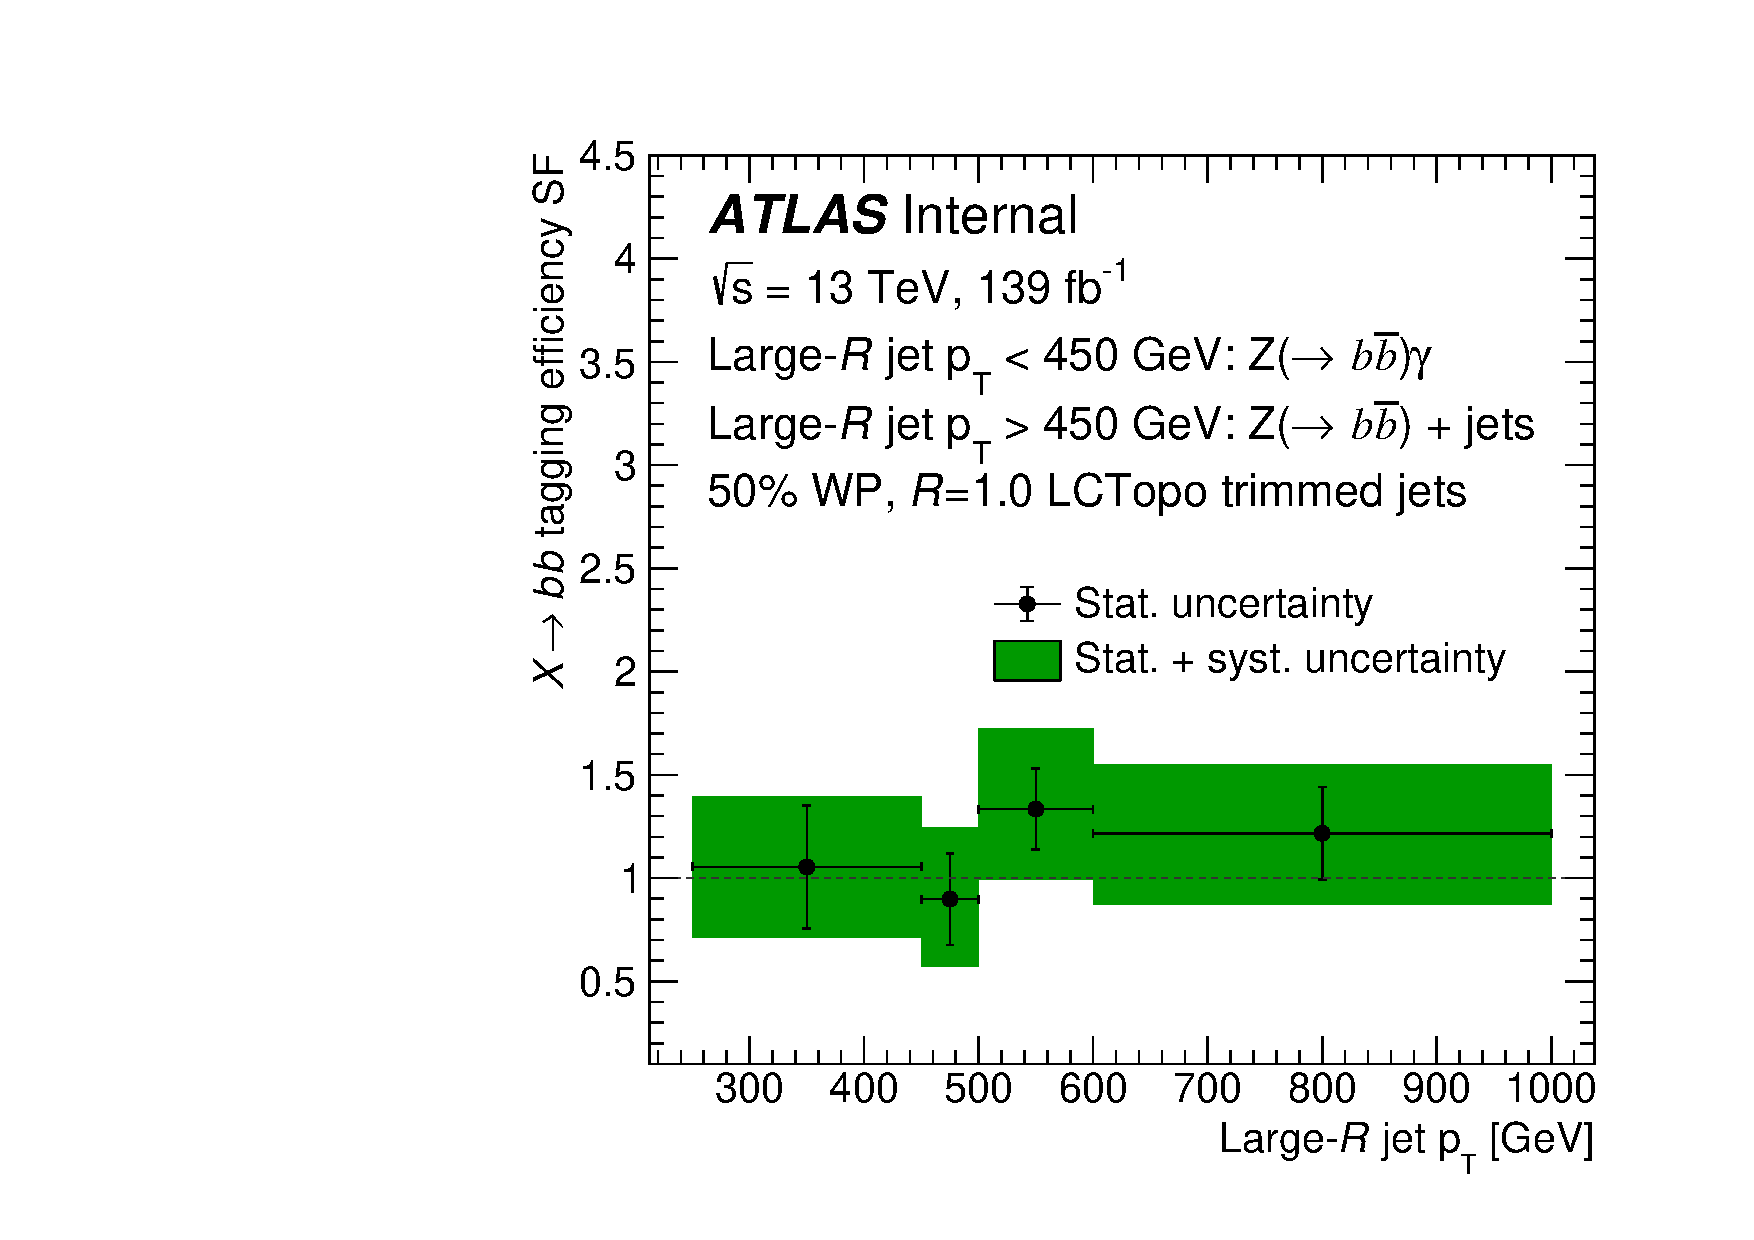
\includegraphics[width=.49\textwidth]{SF_Xbb50_internal_09March2023}}
    \subfigure[]{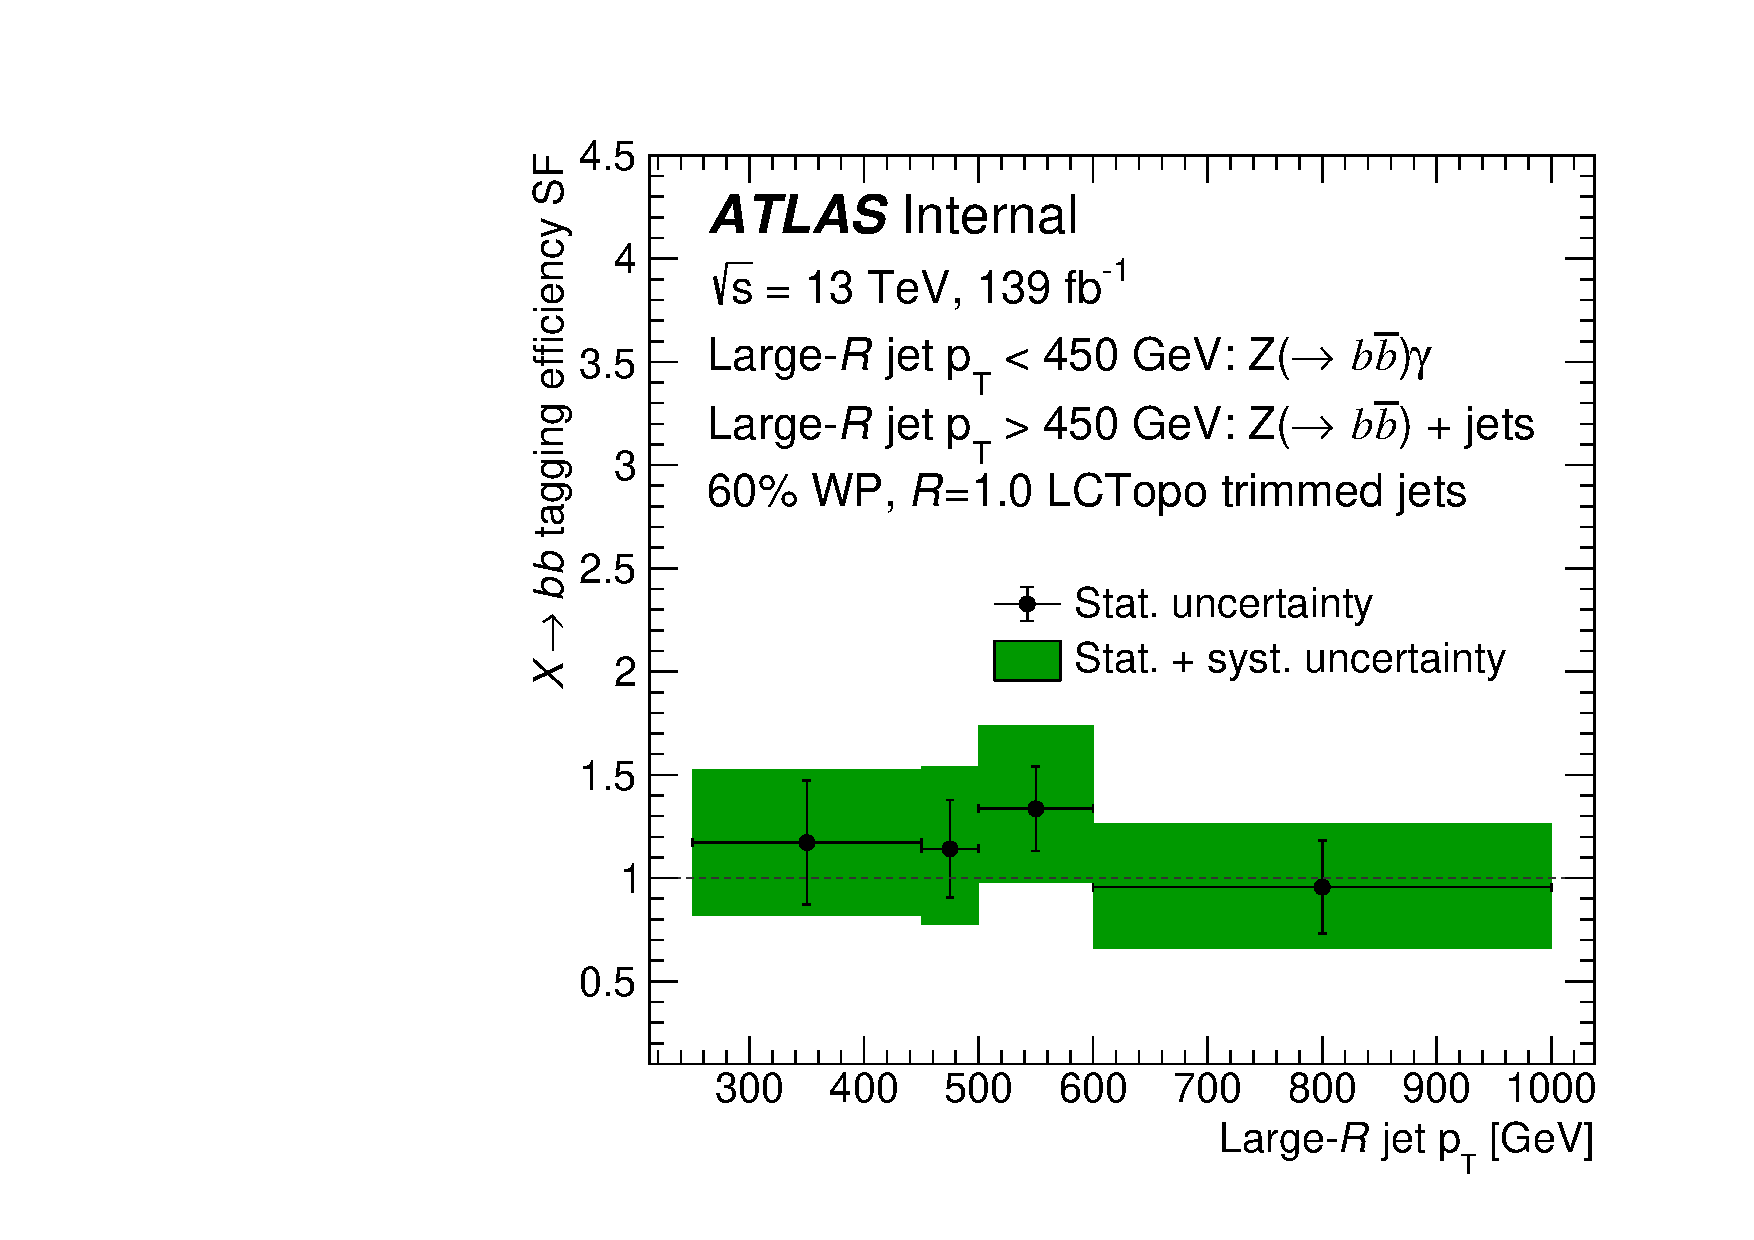
\includegraphics[width=.49\textwidth]{SF_Xbb60_internal_09March2023}}
    \caption[]{Derived scale factors in large-$R$ jet \pt for the \textbf{(a)} \qty[]{50}{\percent} and \textbf{(b)} \qty[]{60}{\percent} \ac{wp} from the calibration of the $X\rightarrow bb$ tagger.}
    \label{fig:xbb_sf}
\end{figure}

\section{Theory Uncertainties}
The cross-section calculation for some process initiated by a proton proton collision calculated at $n$-th order has a functional form \citep{unc_recipe}
\begin{equation}
    \sigma^{(n)} = PDF(x_1, \mu_F)  PDF(x_2, \mu_F) \hat{\sigma}^{(n)}(x_1,x_2,\mu_R),
    \label{eq:xs_unc_1}
\end{equation}
with the \acfp{pdf} carrying momentum fraction $x_{1,2}$ of the partons and the factorization scale $\mu_F$. This scale is named after the assumption that the cross-sections of the initial particle can be calculated by factorizing it in its parton contributions \citep{halzen1984introductory}.
 and depends on the energy as exemplified in figure.
\begin{figure}
    \centering
    \subfigure[]{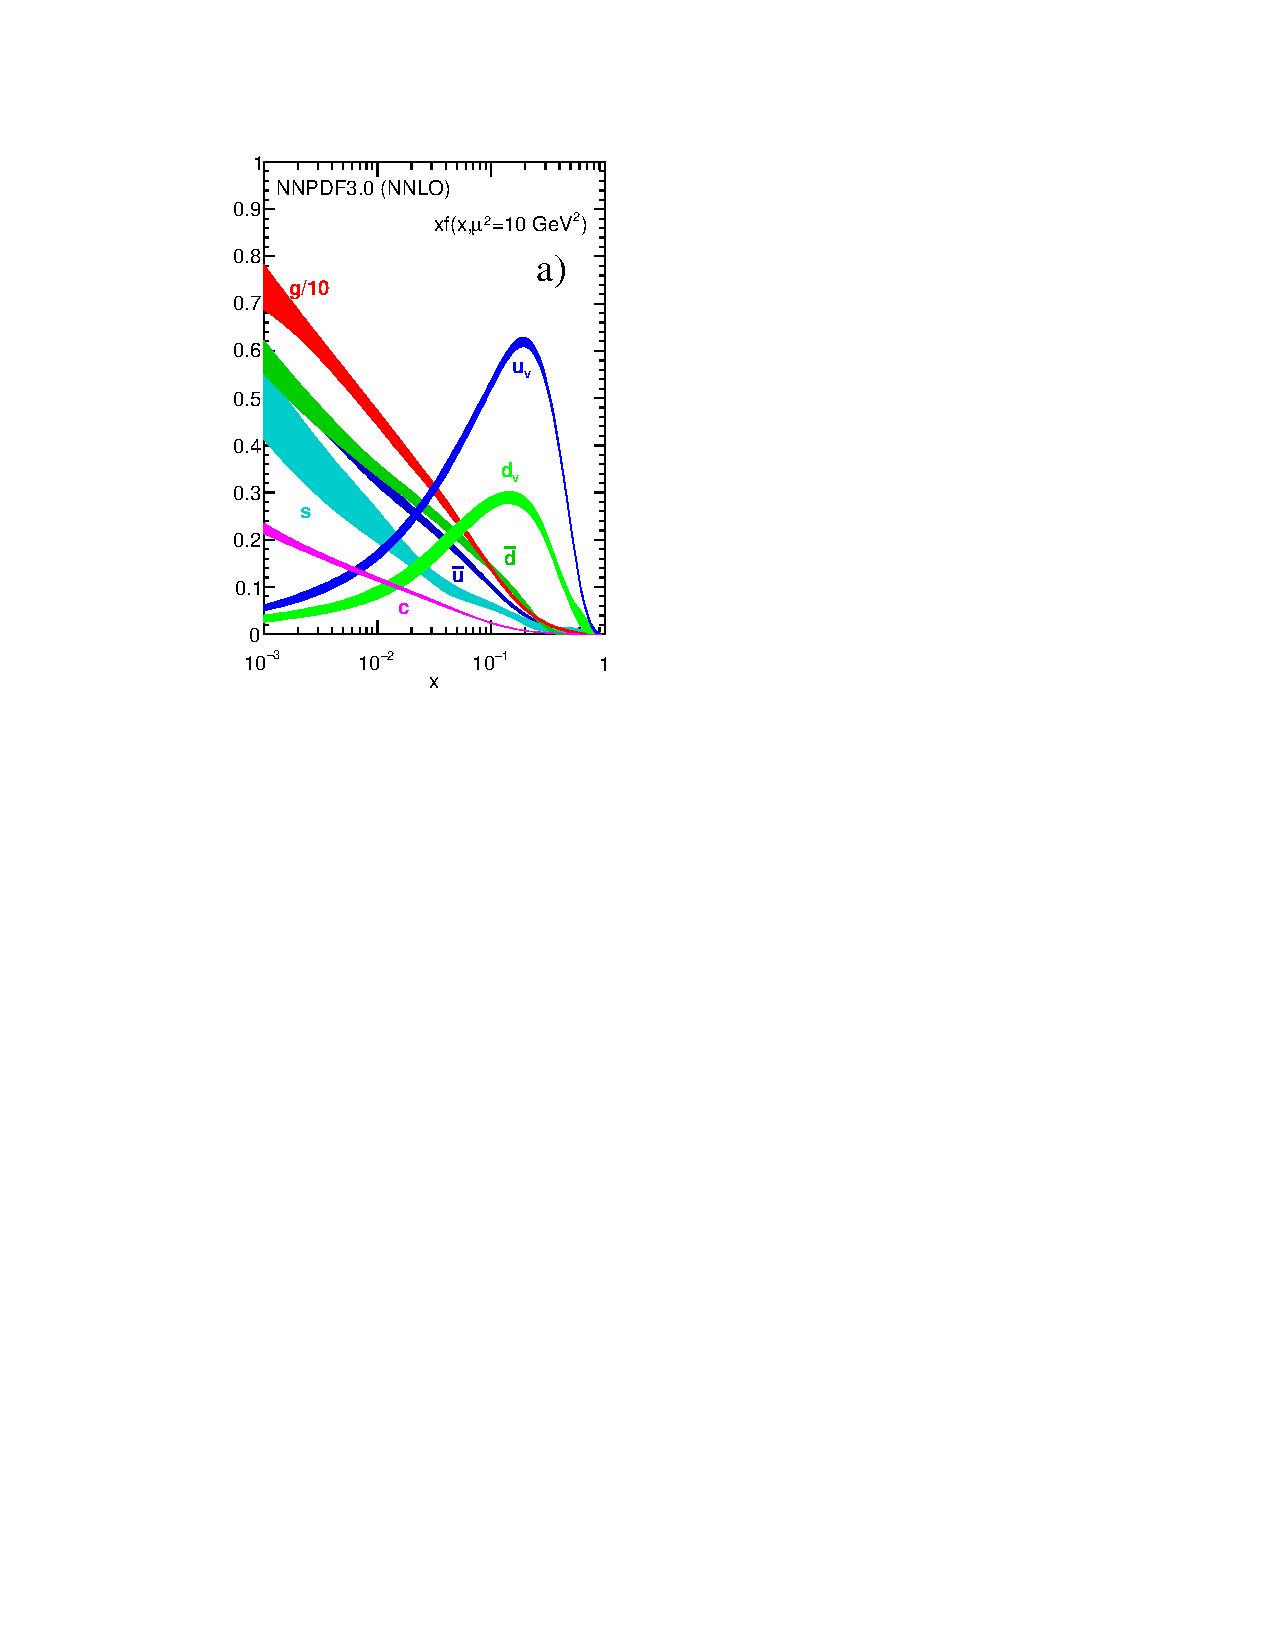
\includegraphics[width=.49\textwidth]{NNPDF-10}}
    \subfigure[]{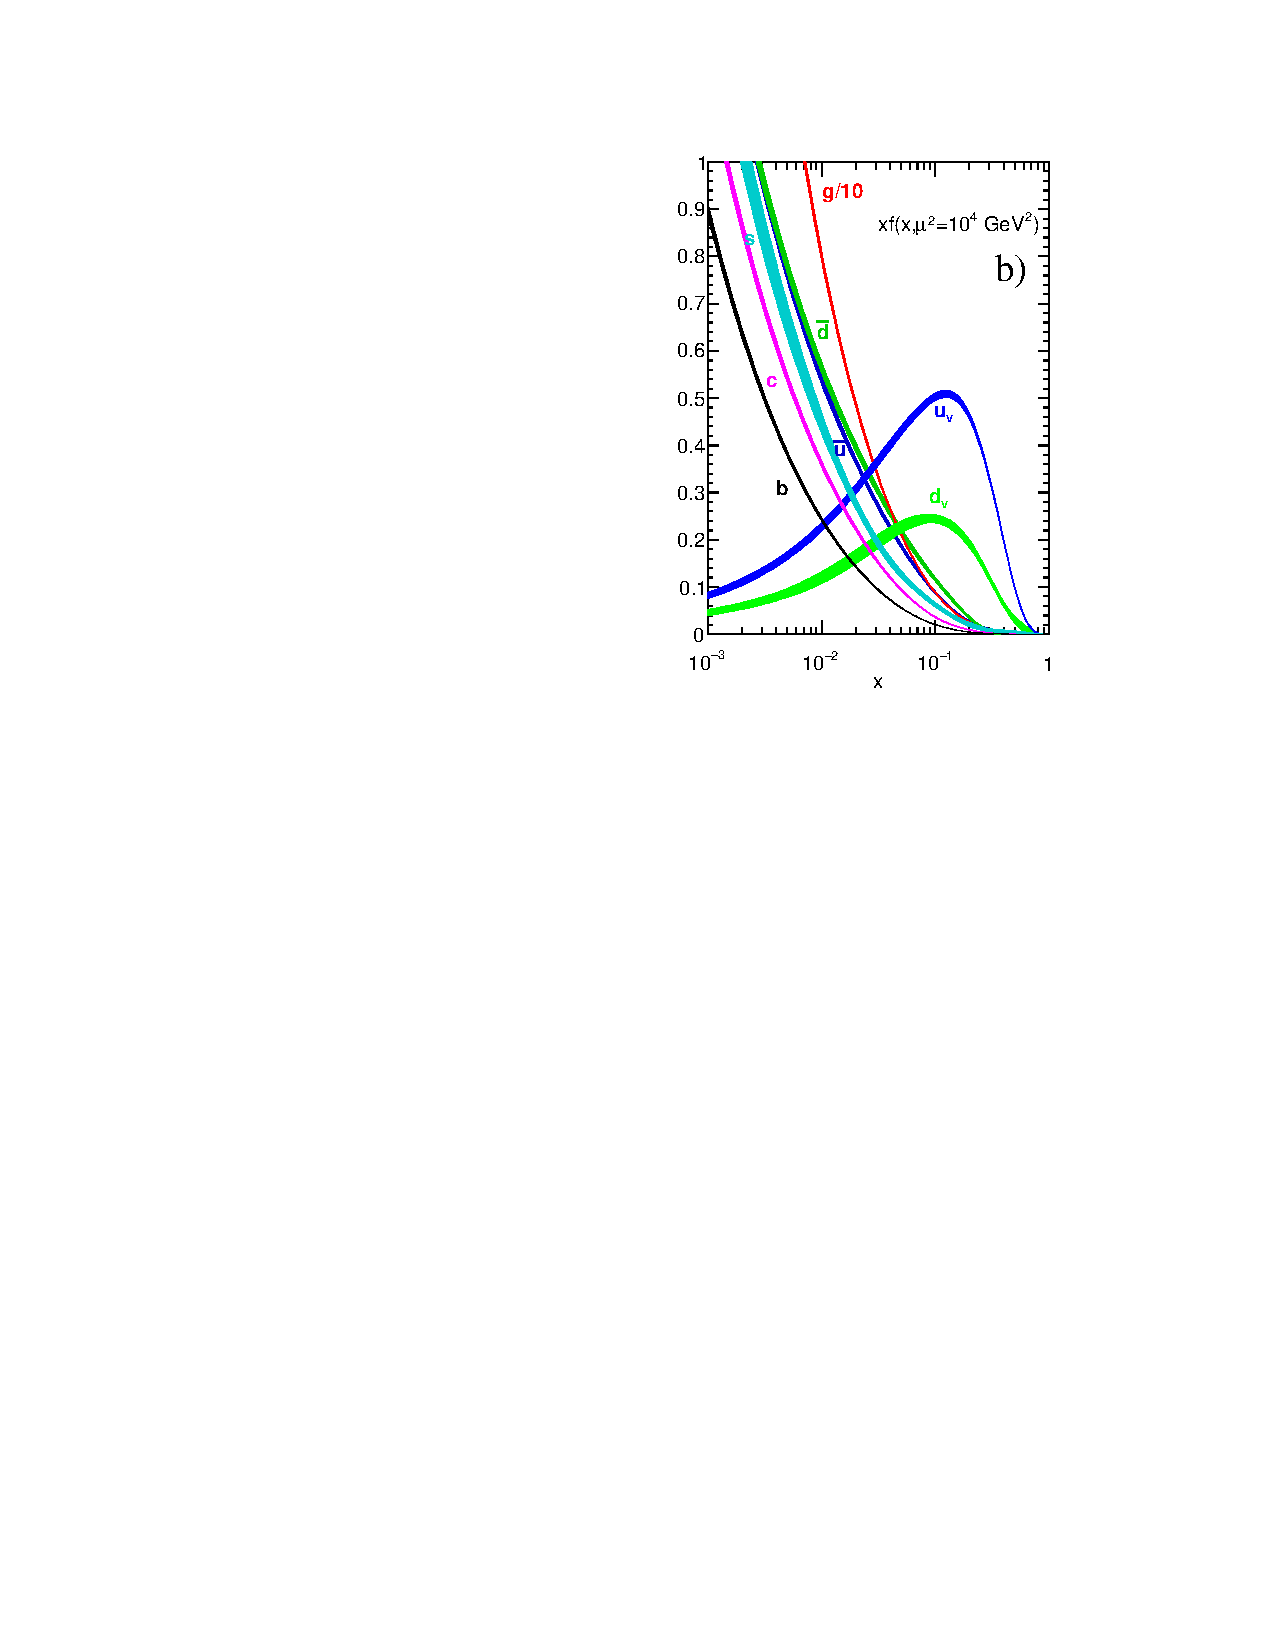
\includegraphics[width=.49\textwidth]{NNPDF-10000}}
    \caption[]{Parton distribution functions for two different factorization scales $\mu_F^2$. (left) $\mu_F^2=$\qty{10}{GeV}$^2$, (right) $\mu_F^2=$\qty{10}{TeV}$^2$. Adopted from \citep{PhysRevD.98.030001}.}
    \label{fig:}
\end{figure}
The term $\hat{\sigma}^{(n)}$ in equation \ref{eq:xs_unc_1} is the calculable part of the cross-section at renormalization scale $\mu_R$ as described in section \ref{sec:renormalization} and is expanded to a desired order $n$ in the strong coupling constant $\alpha_s$ with the usual \ac{qft} ansatz outlined in section \ref{sec:qft}
\begin{equation}
    \hat{\sigma}^{(n)} = \alpha_s \hat{\sigma}^{(0)} + \alpha_s^2 \hat{\sigma}^{(1)} + \ldots + \alpha_s^n \hat{\sigma}^{(n)} + \mathcal{O}(\alpha_s^{n+1}).
    \label{eq:xs_unc_2}
\end{equation}
Modelling cross-sections via \acp{pdf} is necessary since the approximation of the perturbation ansatz of section \ref{sec:qft} breaks down for low energy scales $Q^2$ as described in section \ref{sec:renormalization} which is the energy scale for which the approximation would need to hold to describe the partons inside a proton. However similar to renormalization a scaling behavior can be derived which allows to deduce an estimate of the \acp{pdf} by measuring it at a some energy scale $Q^2$ to extrapolate it to another. The equations enabling this are also expanded in $\alpha_s$ to a desired order and are knwon as DGLAP equations \citep{halzen1984introductory}. Three main sources of uncertainty arise in this calculation described in the following.

\subsubsection*{Scale Variations}
$\alpha_s$ is expanded to some order $n$ in the cross-section calculation and as well in estimating the \acp{pdf}. To account for missing higher orders corrections of theses expansions scale variations of the renormalization and factorization scales are performed pairwise $\{\mu_\text{r},\mu_\text{f}\}\ \times \{0.5,0.5\}, \{1,0.5\}, \{0.5,1\}, \{1,1\}, \{2,1\}, \{1,2\}, \{2,2\}$. For the cross-section calculation this accounts essentially for the term $\mathcal{O}(\alpha_s^{n+1})$ in equation \ref{eq:xs_unc_2}. The envelope that gives the largest variation is taken as the scale uncertainty.

\subsubsection*{\ac{pdf} Uncertainties}
\acp{pdf} need to be deduced from experiment and thus come by themselves with experimental uncertainties. Further uncertainties arise from the functional forms assumed for the \acp{pdf}.

\subsubsection*{$\alpha_s$ Uncertainties}
$\alpha_s$ is also experimentally deduced at the scale of the $Z$ mass which is subject to uncertainties. In all perturbative calculations it is truncated at some order that needs to be accounted for.

The uncertainties on $\alpha_s$ and the \acp{pdf} are both estimated by varying $\alpha_s$. Even though there correlation is not strong they are usually applied combined \citep{unc_recipe}.

\subsection{Uncertainty on HH cross section}
The cross-section calculation for the \ac{vbf} Higgs pair production process has associated uncertainties for the scale variations $^{+0.03\%}_{-0.04\%}$ and the combined \ac{pdf}+$\alpha_s$ uncertainty is $\pm 2.1\%$ \citep{de2016arxiv}.

\subsection{Uncertainty on Acceptance}
Theoretical uncertainties on the final acceptance are evaluated on \ac{mc} simulations for scale variations and \acp{pdf} + $\alpha_s$ \red{TODO, although shouldnt matter...}

% pdf alpha_s easy TODO
\subsection{Parton Shower}
Uncertainties related to the parton showering are estimated using different modelings from \textsc{Pythia 8} and \textsc{Herwig 7}. The largest deviations from the nominal are used as uncertainties on the Higgs pair process. \red{TODO}


\subsection{Branching Ratio Uncertainty}
The error estimate for the branching ratio takes into account theoretical uncertainties (THU) and parametric uncertainties (PU) that are included in the \ac{sm} calculations. The theoretical uncertainties mainly considers missing higher orders while for the parameters $p$ the four leading non-negligible contributions of $p=\alpha_s,m_c,m_b,m_t$ are considered.

Parametric uncertainties are Gaussian errors and are added in quadrature which ensures unity in the Branching Ratio calculation. Theoretical uncertainties in turn are not Gaussian and would lead to underestimated errors and are therefore added linearly \citep{de2016arxiv}. By assuming a Higgs mass of \qty[]{125}{GeV} and considering that there are two Higgs decaying to two $b$-quarks the error on the branching is
\begin{equation}
    \Delta\text{BR} = 2 \times \left(\Delta\text{BR}(\text{THU}) + \sqrt{\sum\nolimits_{p} \Delta\text{BR}(\text{PU}_{p})^2 }\right) = _{-3.5\%}^{+3.4\%}.
\end{equation}

\section{Statistical Uncertainties}
As discussed in the chapter on statistics \ref{sec:statistics} the bin content for histograms in this work follows a Poisson distribution. Therefore the standard error for $N$ events is the square root of the variance $\sigma=\sqrt{\text{Var}}=\sqrt{N}$. Since histograms are filled weighted $\sum_i w_i N_i$ this needs to be taken into account. By making use of the additive property and invariance with respect to constants of the variance a bin filled with weights $w_i$ can be written as
\begin{align}
    \sigma_\text{stat}^2 & = \text{Var}_\text{bin}\left(\sum_i w_i\right)
    =
    \underbrace{\sum_i \text{Var}(w_i \times 1\text{ event})}_{\text{Var}(i+j)=\text{Var}(i)+\text{Var}(j)}
    =
    \underbrace{\sum_i w_i^2\text{Var}(1\text{ event})}_{\text{Var}(aX)=a^2\text{Var}(X)} \\ \nonumber
                         & =\sum_i w_i^2\sqrt{(1\text{ event})},
\end{align}
so that the statistical error reads
\begin{equation}
    \sigma_\text{stat}^\text{bin}=\sqrt{\sum_i w_i^2}.
\end{equation}

\section{Background Derivation Uncertainties}
The \ac{qcd} background is estimated with the ABCD method from the control region as detailed in section \ref{sec:abcd}. The uncertainties are assessed through error propagation of the statistical uncertainty meaning the statistical errors of the event yields used to retrieve the weight factor result in an uncertainty for the weight factor $\Delta w_\text{CR}= \red{\qty[]{0.0}{\percent}}$. To estimate a bin-wise statistical uncertainty of the \ac{nn} score histogram the ABCD procedure is applied in the \ac{vr} by also propagating the error $\Delta w_\text{CR}$ of the applied weight factor.